\chapter{Systematic Error Analysis}
\label{ch:Systs}

As with any analysis, the NC disappearance analysis is sensitive to a number of systematic effects. \nova~was designed with two functionally identical detectors, so that Near Detector data can be used to constrain or correct the Far Detector prediction. Since many effects such as beam and cross section uncertainties affect the spectra at both detectors in a similar or the same way, this two detector technique leads to the reduction of these systematic errors. Other effects, such as Near Detector rock event contamination, require a data driven technique to quantify.

The general technique for analyzing systematic errors was to run the full extrapolation chain and generate a predicted spectrum with and without a systematic effect applied. As in ch.~\ref{ch:Selection}, the prediction assumed the same three flavor oscillation parameters listed in Table \ref{tab:3FlavParams}, and for normalization simplicity, only 14 diblock MC and data were studied. All spectra were then scaled to \pot{6}. Each given systematic effect was used to shift the MC simulation at one or both detectors as appropriate. The resulting difference between the shifted and nominal spectra was quantified as a systematic error.

The systematic effects analyzed included uncertainties arising from the beam, GENIE simulation, Birks-Chou light yield simulation, calibration, bias from the ND containment, ND rock event contamination, ND data/MC spectrum and hadronic energy differences, noise model, MC statistics, and overall normalization. The rest of this chapter discusses each of these effects in greater detail.

\section{Beam}

The \nova~MC simulation involves a fully detailed model of the NuMI beam process in an attempt to create the most realistic MC possible, but systematic errors can result from any mismatch between simulation and reality. The \nova~Beam Working Group performed studies to assess the effect that uncertainties in the simulation can have on the neutrino flux \cite{ref:TNBeam}. These studies included the effects of incorrectly modeling various parts of the beam transport and the effects of uncertainties in hadron production arising from fixed target experiments.

To quantify the systematic error caused by these beam uncertainties, a sample flux was generated using a systematic shift and compared to the nominal flux via a simple ratio. Results were generated separately for each neutrino flavor and for each detector. The ratios were used to modify the MC from the full simulation used as inputs to the extrapolated prediction. Finally, the shifted FD prediction was compared to the nominal prediction, with any differences being taken as the systematic error. At the end of this process, the individual errors were added in quadrature. Errors were calculated for the following systematics:
%\end{doublespace}\begin{singlespace}
\begin{itemize}
  \item Beam position on target varied by $\pm 0.5\,mm$ in X
  \item Beam position on target varied by $\pm 0.5\,mm$ in Y
  \item Beam spot size varied by $\pm 0.2\,mm$ in both X and Y
  \item Target position varied by $+ 2\, mm$ in Z
  \item Horn current varied $\pm 1\,kA$
  \item Horn 1 position varied by $\pm 2\,mm$ in both X and Y
  \item Horn 2 position varied by $\pm 2\,mm$ in both X and Y
  \item Horn magnetic field changed from linear to exponential distribution
  \item Changes to MC beamline simulation
  \item Comparison between versions of FLUKA
  \item Comparison between FLUKA and G4NuMI
  \item Comparison between FLUKA and NA49
\end{itemize}
%\end{singlespace}\begin{doublespace}
\n Hadron production uncertainties were combined in quadrature before being provided as weights, so this is evaluated as single systematic error. The percentage difference due to each systematic is shown in Table \ref{tab:SystBeam}, and the full error envelopes for NC signal and background are shown in Fig.~\ref{fig:SystBeam}. The beam systematics had an overall effect of $3.4\%$ on the NC signal and $8.7\%$ on the background.
\begin{table}[h]
  \begin{center}
    \caption[Beam Systematic Errors]{The percentage difference between the shifted and nominal predictions for the number of FD events due to beam systematics.}
    \label{tab:SystBeam}
    \begin{tabular}{r c c}
      \hline\hline
      Systematic & NC Difference (\%) & Background Difference (\%) \\
      \hline
      Beam Position, X & 0.5 & 0.7 \\
      Beam Position, Y & 0.2 & 0.3 \\
      Beam Spot Size & 0.2 & 0.8 \\
      Target Position & 0.1 & 0.2 \\
      Horn Current & 0.1 & 0.1 \\
      Horn 1 Position & 0.7 & 1.0 \\
      Horn 2 Position & 0.2 & 0.4 \\
      Horn B Field & 0.1 & 0.1 \\
      Geometry Simulation Change & 0.4 & 2.1 \\
      FLUKA Versions & 0.04 & 0.6 \\
      FLUKA v G4NuMI & 0.4 & 3.0 \\
      FLUKA v NA49 & 3.3 & 9.3 \\
      \hline
      Combined & 3.6 & 10.4 \\
      \hline
    \end{tabular}
  \end{center}
\end{table}

\begin{figure}[h]
  \centering
  \begin{subfigure}{.48\textwidth}
    \centering
    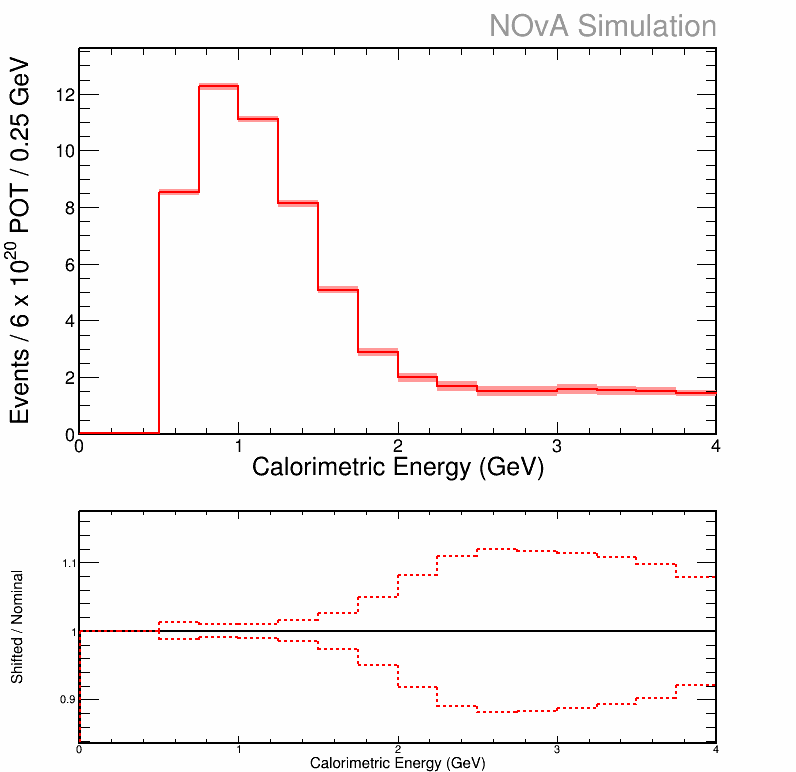
\includegraphics[width=1\linewidth]{figures/cNCEXBeamSysts.png}
  \end{subfigure}
  \begin{subfigure}{.48\textwidth}
    \centering
    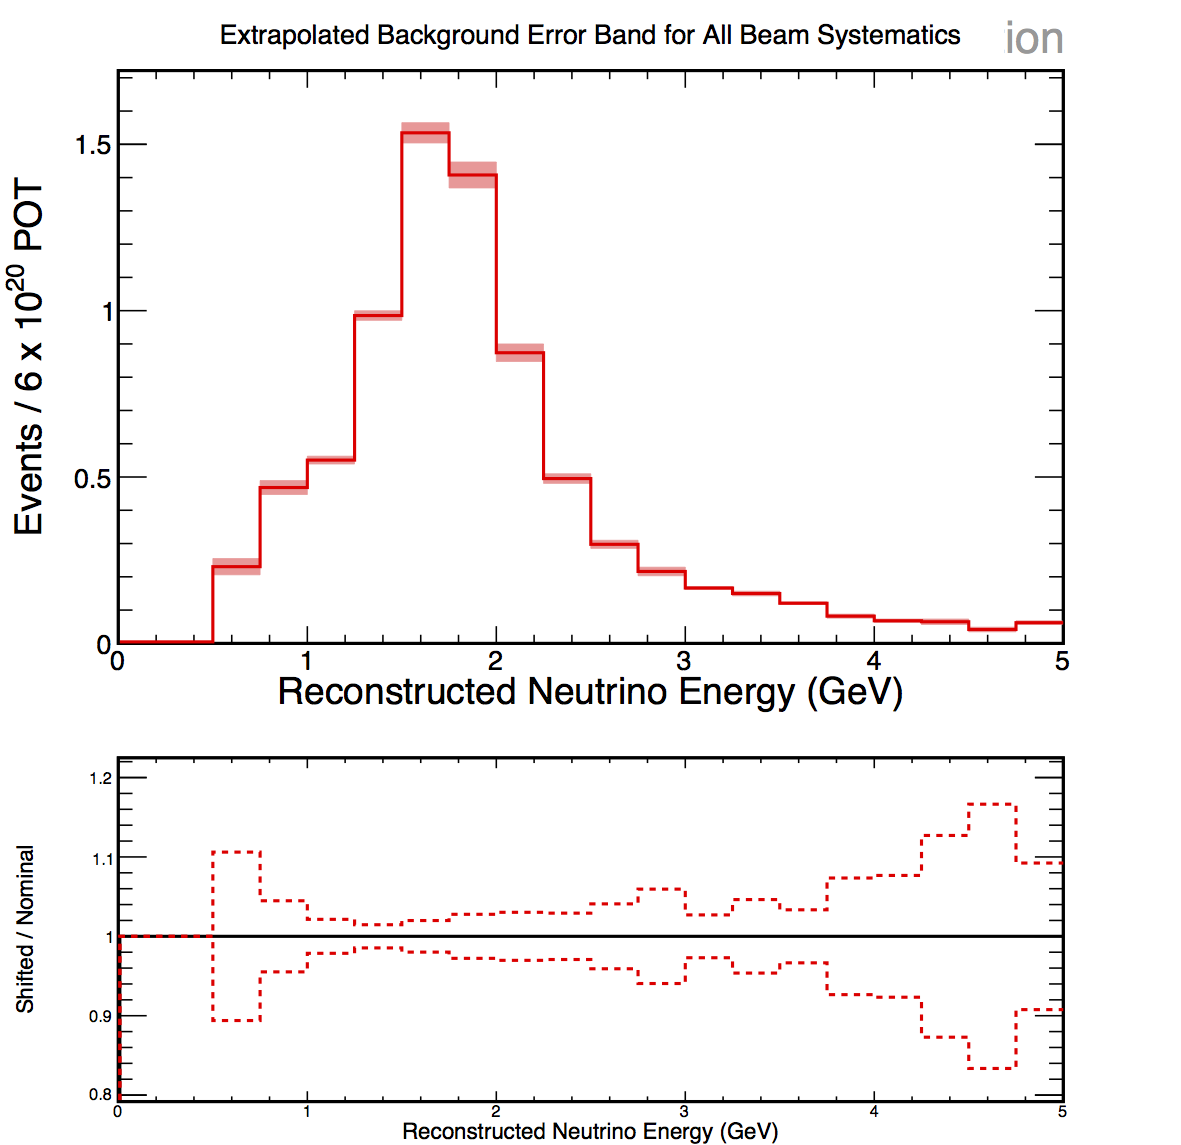
\includegraphics[width=1\linewidth]{figures/cBGEXBeamSysts.png}
  \end{subfigure}
  \caption[Beam Systematic Error Envelopes]{Systematic error envelope on the NC signal (left) and background (right) event spectra, after extrapolation. The envelope was calculated by adding in quadrature the larger of $\vert +1\sigma \vert$ and $\vert -1\sigma \vert$ for each individual systematic.}
  \label{fig:SystBeam}
\end{figure}

\section{Birks-Chou Light Yield Simulation}

The \nova~MC simulation employs the Birks-Chou Law to model the relationship between scintillator light yield, $LY$, and particle energy deposition rate, $\frac{dE}{dx}$ \cite{ref:BirksChou}. 
\beq
LY = A \frac{ \frac{dE}{dx} }{1 + k_B \frac{dE}{dx} + k_C \left( \frac{dE}{dx} \right)^2} 
\label{eq:BirksChou}
\eeq

\n This formula encapsulates the known light yield quenching that occurs for particles with a high energy deposition rate. The constants $k_B$ and $k_C$ are dependent on the scintillator material and had to be estimated for \nova~as no measurement existed for the particular material used in this experiment. A study was performed comparing the energy deposition at the end of proton tracks in the ND for both data and MC to find parameters that would generate agreement between the two \cite{ref:DanBirks}. The results of the study were $k_B = 0.04\unit{cm/MeV}$ and $k_C = -0.0005\unit{(cm/MeV)}^2$.

The systematic error based on the Birks-Chou light yield simulation was quantified by comparing the nominal FD prediction to predicted spectra using alternative Birks-Chou parameter constants. The values reported in the study from \cite{ref:DanBirks} were much larger than other typical measurements, so two MC samples were generated with more traditional values, one with $k_B = 0.01\unit{cm/MeV}$ called BirksB, the other with $k_B = 0.02\unit{cm/MeV}$ called BirksC, both with $k_C = 0$. Shifted FD event spectra were predicted by extrapolating the same set of ND data as the nominal prediction, but using the MC with alternative Birks-Chou model parameters. The error was taken as the percentage difference between the nominal and shifted predictions. Table \ref{tab:SystBirks} shows the percentage differences from both MC samples; fig.~\ref{fig:SystBirks} shows the shifted event spectra compared to nominal. Instead of combining the individual errors in quadrature, the shifted sample with the larger overall difference from the BirksB model taken as the systematic error, which had a $2.9\%$ effect on the NC signal, and a $3.1\%$ effect on the background.
\begin{table}[h]
  \begin{center}
    \caption[Birks-Chou Systematic Errors]{The percentage difference between the shifted and nominal predictions for the number of FD events due to extrapolation using MC with alternative Birks-Chou model parameters.}
    \label{tab:SystBirks}
    \begin{tabular}{r c c}
      \hline\hline
      Model & NC Difference (\%) & Background Difference (\%) \\
      \hline
      BirksB & 2.9 & 1.6 \\
      BirksC & 3.1 & 4.5 \\
      \hline
    \end{tabular}
  \end{center}
\end{table}

\begin{figure}[h]
  \centering
  \begin{subfigure}{.48\textwidth}
    \centering
    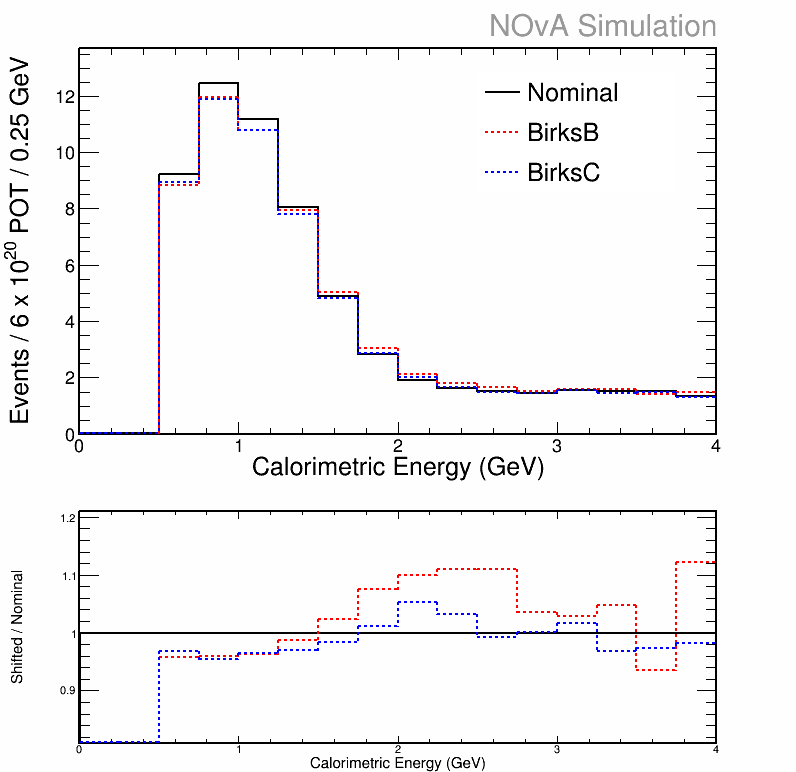
\includegraphics[width=1\linewidth]{figures/cNCEXBirksSysts.png}
  \end{subfigure}
  \begin{subfigure}{.48\textwidth}
    \centering
    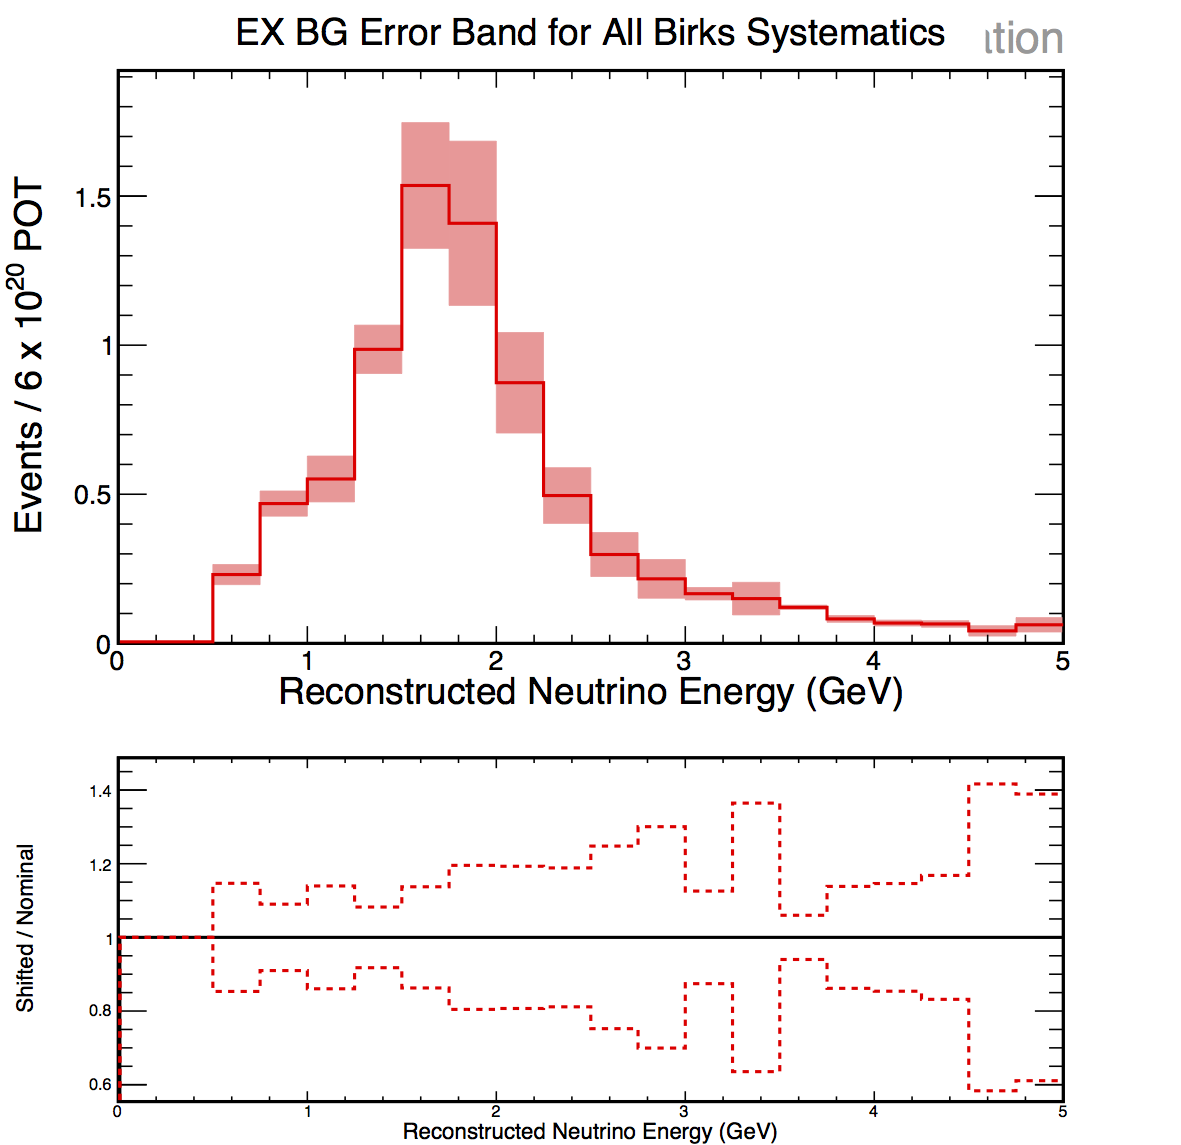
\includegraphics[width=1\linewidth]{figures/cBGEXBirksSysts.png}
  \end{subfigure}
  \caption[Birks-Chou Shifted FD Predictions]{Shifted FD predictions due to extrapolation of ND data with MC using different Birks-Chou parameter values. The NC signal spectrum is on the left; the background spectrum is on the right.}
  \label{fig:SystBirks}
\end{figure}

\section{Calibration}

The calibration procedure is designed to make a constant energy response both across each detector and between the two, but any problem can introduce a systematic error. This error was evaluated by studying various MC samples with an engineered miscalibration. The effects studied included a miscalibration that varied as a function of the cell length and an overall scale miscalibration. The functional miscalibration was studied separately between the X and Y views of the detector. The scale miscalibration was applied as a 5\% effect both up and down at each detector. These effects are motivated by studying data/MC comparisons for various samples \cite{ref:TNCalib, ref:CalibMESA, ref:CalibPi0SA} and were updated based on the most recent round of data \cite{ref:CalibSA}.

The systematic error was evaluated in two regimes. The first applied the same miscalibration to the MC at both detectors, and a shifted prediction was then generated using these shifted as inputs into the extrapolation. This procedure was followed for each type of miscalibration, and all of these systematics were added in quadrature at the end. The overall scale miscalibration was also applied as a miscalibration to a single detector to measure the effect of a missed absolute calibration. A shifted prediction was then generated as above, but with this procedure only the maximum overall effect was used as the systematic error that was then added in quadrature with the systematics from above. Table \ref{tab:SystCalib} shows the percentage difference for each of the calibration systematics. The overall error was $TODO\%$ on the NC signal and $TODO\%$ on the background.
\begin{table}[h]
  \begin{center}
    \caption[Calibration Systematic Errors]{The percentage difference between the shifted and nominal predictions for the number of FD events due to deliberately applied miscalibrations. For the flat scale miscalibration applied to 1 detector, the largest overall effect from the scale TODO at the ND was taken as the systematic.}
    \label{tab:SystCalib}
    \begin{tabular}{r c c}
      \hline\hline
      Miscalibration & NC Difference (\%) & Background Difference (\%) \\
      \hline
      \multicolumn{3}{l}{Miscalibration applied to both detectors:} \\
      Sloped X & & \\
      Sloped Y & & \\
      Flat Scale Up & & \\
      Flat Scale Down & & \\
      \multicolumn{3}{l}{Miscalibration applied to one detector:} \\
      Flat Scale Up, ND & & \\
      Flat Scale Down, ND & & \\
      Flat Scale Up, FD & & \\
      Flat Scale Down, FD & & \\
      \hline
    \end{tabular}
  \end{center}
\end{table}

\section{GENIE Simulation}

Neutrino interactions in the \nova~simulation are generated using GENIE \cite{ref:GENIE}, a generator that involves a detailed physics modeling of cross sections, hadronization, and final state interactions. GENIE includes a plethora of parameters that alter individual physics input quantities, with the parameters themselves acting as systematic uncertainties, either dialing up or down a particular quantity by a standard deviation recommended by the GENIE authors.

The systematic uncertainties from physics modeling were evaluated by using the GENIE parameters as event reweights. Nominal MC was produced using the parameters and weights as provided by the GENIE authors, but also included a table of weights to modify an events `worth' based on how much the different GENIE parameters shifted. Using the reweight table, a nominal FD prediction was produced from the default MC, and a shifted prediction was produced for each of the parameters provided by GENIE. The percentage difference was taken as the systematic error for the particular parameter. Table \ref{tab:SystGENIE} lists all of the parameters considered for the systematic study, and the associated error. Fig.~\ref{fig:SystGENIE} shows the final systematic error envelope. The combined systematic error, adding the individual contributions in quadrature, was $11.3\%$ for the NC signal and $12.8\%$ for the background.

\singlespacing
\begin{longtable}{p{3in} c @{\hskip 0.25in} c c}
  \caption[GENIE Systematic Errors]{The systematic error, in percentage difference, for each GENIE systematic parameter. The description and standard deviations come from ref.~\cite{ref:GENIE, ref:TNGENIE}. Parameters with a standard deviation marked as `D' are discrete and thus do not have a standard deviation estimate.} \tabularnewline
  \hline\hline
  \multicolumn{2}{c}{Parameter Description and Standard Deviation} & NC Diff. (\%) & Bkg.~Diff. (\%) \\
  \hline \endfirsthead
  \hline\hline
  \multicolumn{2}{c}{Parameter Description and Standard Deviation} & NC Diff. (\%) & Bkg.~Diff. (\%) \\
  \hline \endhead
  Axial mass for NC elastic & $\pm25\%$ & 1.7 & 0.8 \\
  Strange axial form factor $\eta$ for NC elastic & $\pm30\%$ & 0.04 & 0.02 \\
  Normalization Factor for CCQE & $^{+25\%}_{-15\%}$ & 0.5 & 1.2 \\
  Axial mass CCQE distribution shape & $^{+25\%}_{-15\%}$ & 0.2 & 0.3 \\
  CCQE Pauli suppression (via changes in Fermi level $k_F$) & $\pm35\%$ & 0.02 & 0.1 \\
  Choice of CCQE vector form factors \newline (BBA05 $\leftrightarrow$ Dipole) & D & 0.1 & 0.2 \\
%  Parametrization of nucleon momentum distributions & D & 0.00 & 0.00 \\ %CCQEMomDistroFGtoSF
  Axial mass for CC resonance neutrino production & $\pm20\%$ & 4.4 & 8.2 \\
  Vector mass for CC resonance neutrino production & $\pm10\%$ & 2.6 & 4.5 \\
  Axial mass for NC resonance neutrino production & $\pm20\%$ & 7.3 & 3.9 \\
  Vector mass for NC resonance neutrino production & $\pm10\%$ & 1.9 & 0.9 \\
  Axial mass for CC and NC coherent pion \newline production & $\pm50\%$ & 1.1 & 0.3 \\
  Nuclear size param controlling $\pi$ absorption in RS model & $\pm10\%$ & 1.0 & 0.3 \\
  Non-resonance bkg in $\nu p$ CC$1\pi$ reactions & $\pm50\%$ & 0.5 & 1.1 \\
  Non-resonance bkg in $\nu p$ CC$2\pi$ reactions & $\pm50\%$ & 1.2 & 2.5 \\
  Non-resonance bkg in $\nu n$ CC$1\pi$ reactions & $\pm50\%$ & 1.9 & 4.1 \\
  Non-resonance bkg in $\nu n$ CC$2\pi$ reactions & $\pm50\%$ & 1.2 & 2.5 \\
  Non-resonance bkg in $\nu p$ NC$1\pi$ reactions & $\pm50\%$ & 0.7 & 0.4 \\
  Non-resonance bkg in $\nu p$ NC$2\pi$ reactions & $\pm50\%$ & 2.0 & 1.4 \\
  Non-resonance bkg in $\nu n$ NC$1\pi$ reactions & $\pm50\%$ & 1.9 & 1.2 \\
  Non-resonance bkg in $\nu n$ NC$2\pi$ reactions & $\pm50\%$ & 1.0 & 0.8 \\
  Non-resonance bkg in $\bar{\nu} p$ CC$1\pi$ reactions & $\pm50\%$ & 0.01 & 0.1 \\
  Non-resonance bkg in $\bar{\nu} p$ CC$2\pi$ reactions & $\pm50\%$ & 0.01 & 0.04 \\
  Non-resonance bkg in $\bar{\nu} n$ CC$1\pi$ reactions & $\pm50\%$ & 0.00 & 0.00 \\
  Non-resonance bkg in $\bar{\nu} n$ CC$2\pi$ reactions & $\pm50\%$ & 0.01 & 0.02 \\
  Non-resonance bkg in $\bar{\nu} p$ NC$1\pi$ reactions & $\pm50\%$ & 0.1 & 0.1 \\
  Non-resonance bkg in $\bar{\nu} p$ NC$2\pi$ reactions & $\pm50\%$ & 0.1 & 0.04 \\
  Non-resonance bkg in $\bar{\nu} n$ NC$1\pi$ reactions & $\pm50\%$ & 0.03 & 0.02 \\
  Non-resonance bkg in $\bar{\nu} n$ NC$2\pi$ reactions & $\pm50\%$ & 0.1 & 0.1 \\
  $A_{HT}$ higher-twist param in BY model scaling variable $\xi_w$ & $\pm25\%$ & 0.1 & 0.1 \\
  $B_{HT}$ higher-twist param in BY model scaling variable $\xi_w$ & $\pm25\%$ & 0.1 & 0.2 \\
  $C_{V1u}$ u valence GRV98 PDF correction param in BY model & $\pm30\%$ & 0.1 & 0.1 \\
  $C_{V2u}$ u valence GRV98 PDF correction param in BY model & $\pm40\%$ & 0.1 & 0.1 \\
%  Inclusive CC cross-section normalization factor & 0.00 & 0.00 & \\
%  $\bar{\nu}/\nu$ CC ratio & 0.00 & 0.00 & \\
%  DIS nuclear & 0.00 & 0.00 & \\
  Pion transverse momentum ($p_T$) for $N\pi$ states in AGKY & D & 0.01 & 0.01 \\
  Pion Feynman x ($x_F$) for $N\pi$ states in AGKY & D & 0.01 & 0.03 \\
%  Hadron formation zone & $\pm50\%$ & 0.00 & 0.00 \\
  Pion angular distribution in $\Delta \rightarrow \pi N$ \newline (isotropic $\leftrightarrow$ RS) & D & 0.3 & 0.2 \\
  Branching ratio for radiative resonance decays & $\pm50\%$ & 0.03 & 0.01 \\
  Branching ratio for single-$\eta$ resonance decays & $\pm50\%$ & 0.2 & 0.2 \\
  Nucelon mean free path (total rescattering \newline probability) & $\pm20\%$ & 0.3 & 0.9 \\
  Nucleon charge exchange probability & $\pm50\%$ & 0.1 & 0.2 \\
  Nucleon elastic reaction probability & $\pm30\%$ & 0.3 & 0.5 \\
  Nucleon inelastic reaction probability & $\pm40\%$ & 0.1 & 0.1 \\
  Nucleon absorption probability & $\pm20\%$ & 0.2 & 0.2 \\
  Nucleon $\pi$-production probability & $\pm20\%$ & 0.03 & 0.1 \\
  $\pi$ mean free path (total rescattering probability) & $\pm20\%$ & 0.7 & 0.9 \\
  $\pi$ charge exchange probability & $\pm50\%$ & 0.1 & 0.2 \\
  $\pi$ elastic reaction probability & $\pm10\%$ & 0.2 & 0.1 \\
  $\pi$ inelastic reaction probability & $\pm40\%$ & 0.1 & 0.1 \\
  $\pi$ absorption probability & $\pm20\%$ & 1.0 & 0.6 \\
  $\pi$ $\pi$-production probability & $\pm20\%$ & 0.04 & 0.1 \\
  MEC event scale & $+50\%$ & 0.3 & 0.2 \\
  RPA event weight & Varied & 0.1 & 0.4 \\
  \hline
  Combined & & 11.3 & 12.8 \\
  \hline
  \label{tab:SystGENIE}
\end{longtable}
\doublespacing

\begin{figure}[h]
  \centering
  \begin{subfigure}{.48\textwidth}
    \centering
    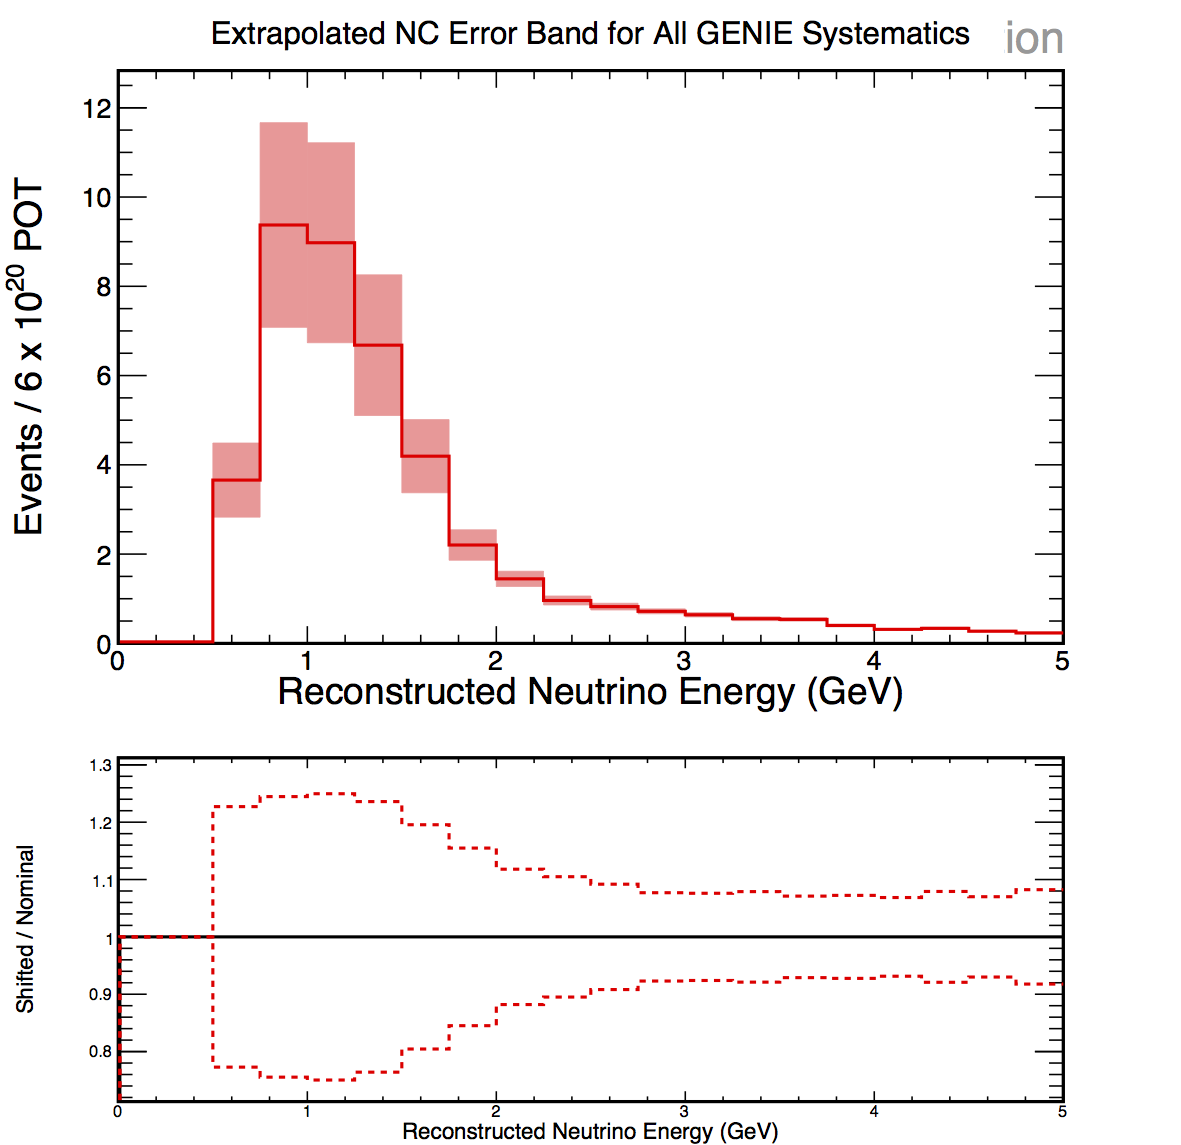
\includegraphics[width=1\linewidth]{figures/cNCEXGENIESysts.png}
  \end{subfigure}
  \begin{subfigure}{.48\textwidth}
    \centering
    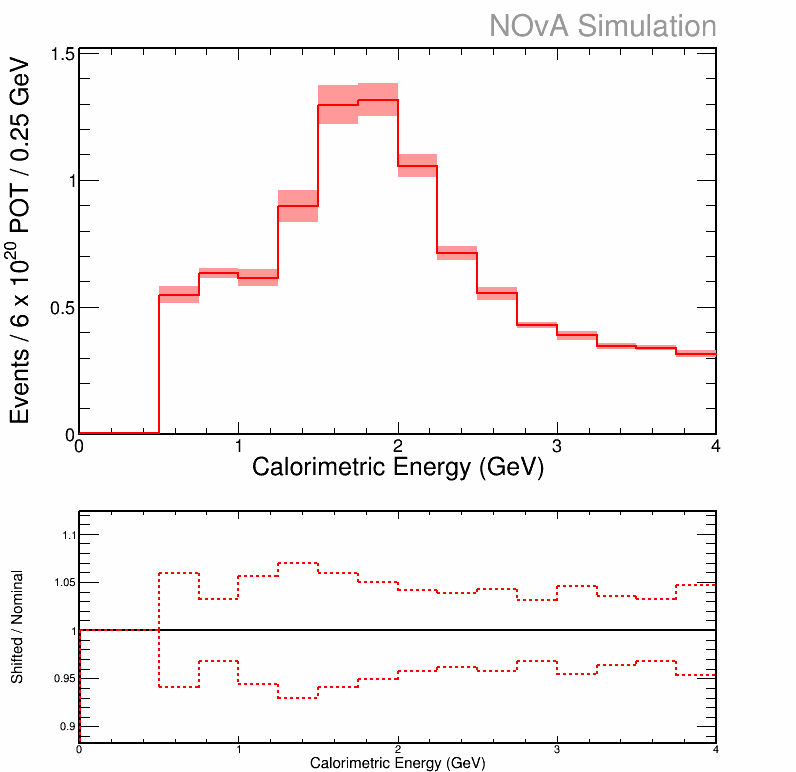
\includegraphics[width=1\linewidth]{figures/cBGEXGENIESysts.png}
  \end{subfigure}
  \caption[GENIE Systematic Error Envelopes]{Systematic error envelope on the NC signal (left) and background (right) event spectra, after extrapolation. The envelope was calculated by adding in quadrature the larger of $\vert +1\sigma \vert$ and $\vert -1\sigma \vert$ for each individual systematic.}
  \label{fig:SystGENIE}
\end{figure}

\section{ND Containment}

The ND does not see an effective point source of neutrinos like the FD due to its proximity to the beam source. As a result, the neutrino flux is not uniform across the detector, and so the energy spectrum of neutrinos seen by the two \nova~detectors is slightly different. To study the effect this has on the extrapolated prediction, multiple predicted FD spectra were generated using subsamples of the ND. The fiducial volume of the ND was split in half along each axis, and split into an inner and outer half (the overall containment criteria was left in tact). The extrapolation was performed using each of these `half detectors.' The error was taken as the percentage difference from the shifted prediction to the nominal. Table \ref{tab:SystFidCont} shows the results from each of these extrapolations and fig.~\ref{fig:SystFidCont} show the shifted spectra. Like the Birks-Chou systematic, the largest overall difference was taken as the systematic error for a $3.6\%$ effect on the NC signal and a $3.0\%$ effect on the background.
\begin{table}[h]
  \begin{center}
    \caption[ND Containment Systematic Errors]{The percentage difference between the shifted and nominal predictions for the number of FD events after extrapolation using half of the fiducial volume at the ND.}
    \label{tab:SystFidCont}
    \begin{tabular}{r c c}
      \hline\hline
      ND Half & NC Difference (\%) & Background Difference (\%) \\
      \hline
      West (+X) & 0.1 & 0.6 \\
      East (-X) & 0.03 & 0.5 \\
      Top (+Y) & 1.1 & 0.6 \\
      Bottom (-Y) & 1.2 & 0.7 \\
      Front (Low Z) & 0.7 & 0.4 \\
      Back (High Z) & 0.7 & 0.4 \\
      Inner (Low $\vert$X$\vert$, $\vert$Y$\vert$) & 1.3 & 0.8 \\
      Outer (High $\vert$X$\vert$, $\vert$Y$\vert$) & 3.6 & 3.0 \\
      \hline
    \end{tabular}
  \end{center}
\end{table}

\begin{figure}[h]
  \centering
  \begin{subfigure}{.48\textwidth}
    \centering
    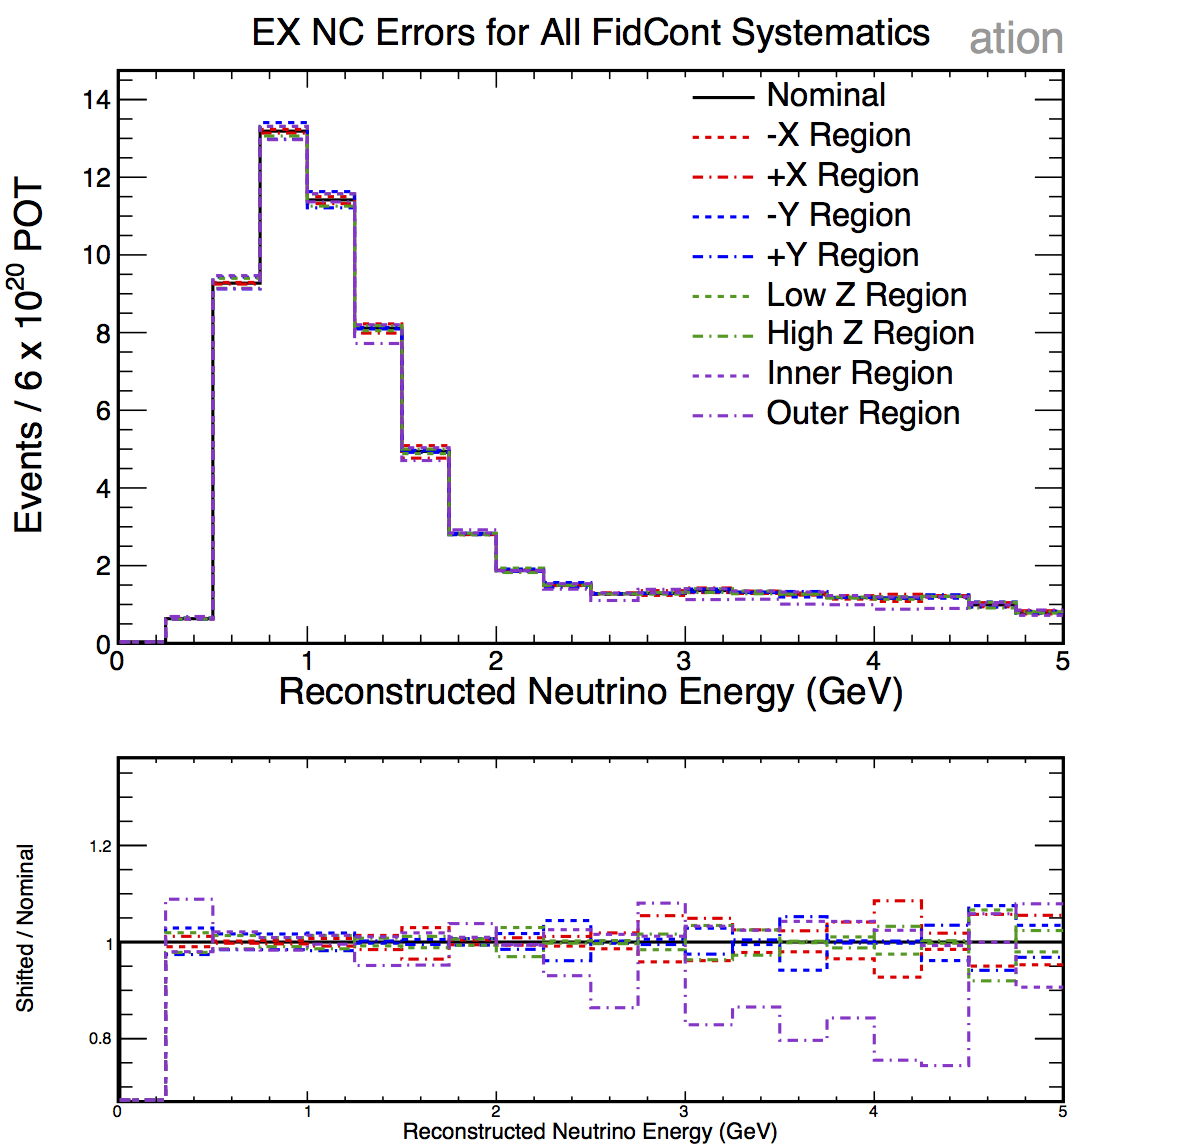
\includegraphics[width=1\linewidth]{figures/cNCEXFidContSysts.png}
  \end{subfigure}
  \begin{subfigure}{.48\textwidth}
    \centering
    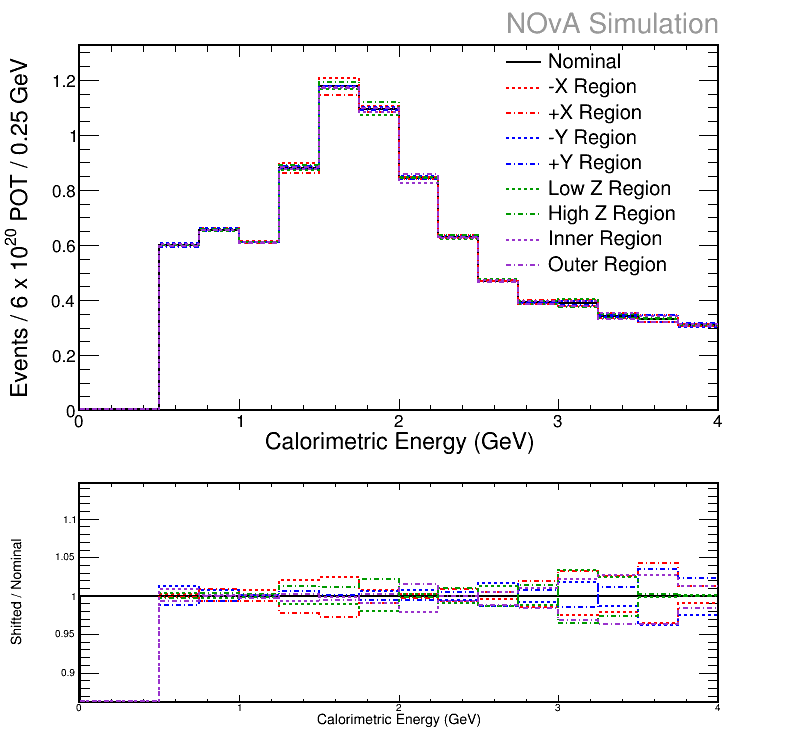
\includegraphics[width=1\linewidth]{figures/cBGEXFidContSysts.png}
  \end{subfigure}
  \caption[Shifted FD Predictions from Extrapolation of Halves of the ND]{Shifted FD predictions after extrapolation using only half of the ND fiducial volume. The NC signal spectrum is on the left; the background spectrum is on the right.}
  \label{fig:SystFidCont}
\end{figure}

\section{ND Rock Event Contamination}

The MC simulation does include neutrino interactions that occur in the rock that surrounds the ND. These events often leak into the detector volume, and while most of them are cut away by fiducial and containment cuts, there are some that remain. Those events that do remain cannot be reconstructed properly as their origins are outside of the detector. 

The systematic error that is incurred due to the rock event contamination was estimated by predicting the FD event spectrum from an extrapolation with rock events removed by MC truth and comparing to the nominal predicted spectrum. The events were only removed from the ND MC sample, requiring that the true neutrino vertex was inside the detector to remain. The shifted spectra are shown in Fig.~\ref{fig:SystNDRock}. This systematic amounted to an overall $4.4\%$ shift on the NC signal spectrum and a $1.5\%$ shift on the background spectrum.

\begin{figure}[h]
  \centering
  \begin{subfigure}{.48\textwidth}
    \centering
    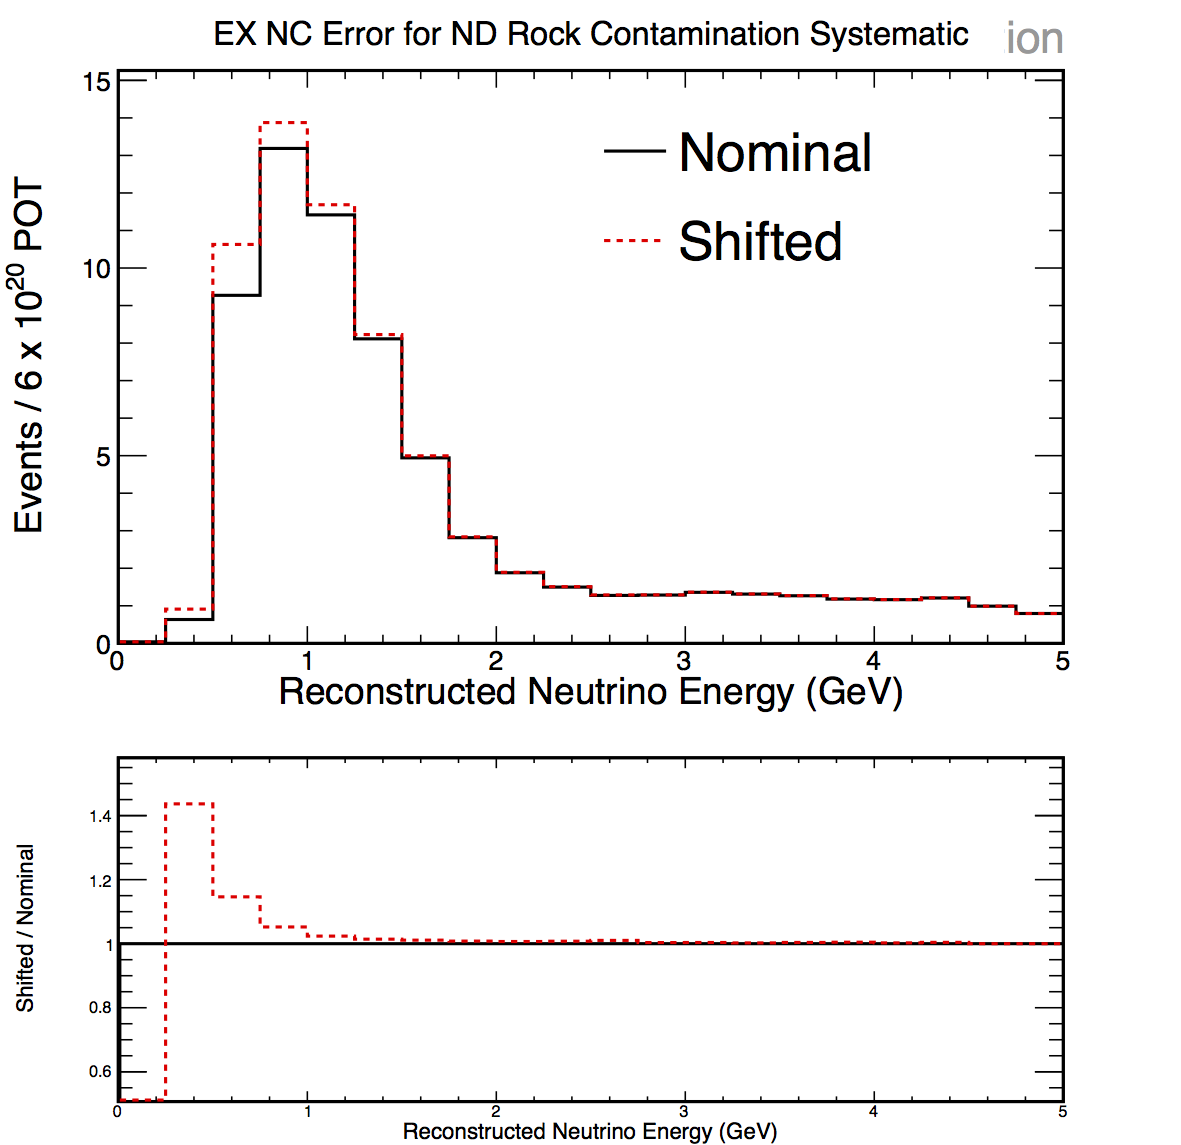
\includegraphics[width=1\linewidth]{figures/cNCEXNDRockSysts.png}
  \end{subfigure}
  \begin{subfigure}{.48\textwidth}
    \centering
    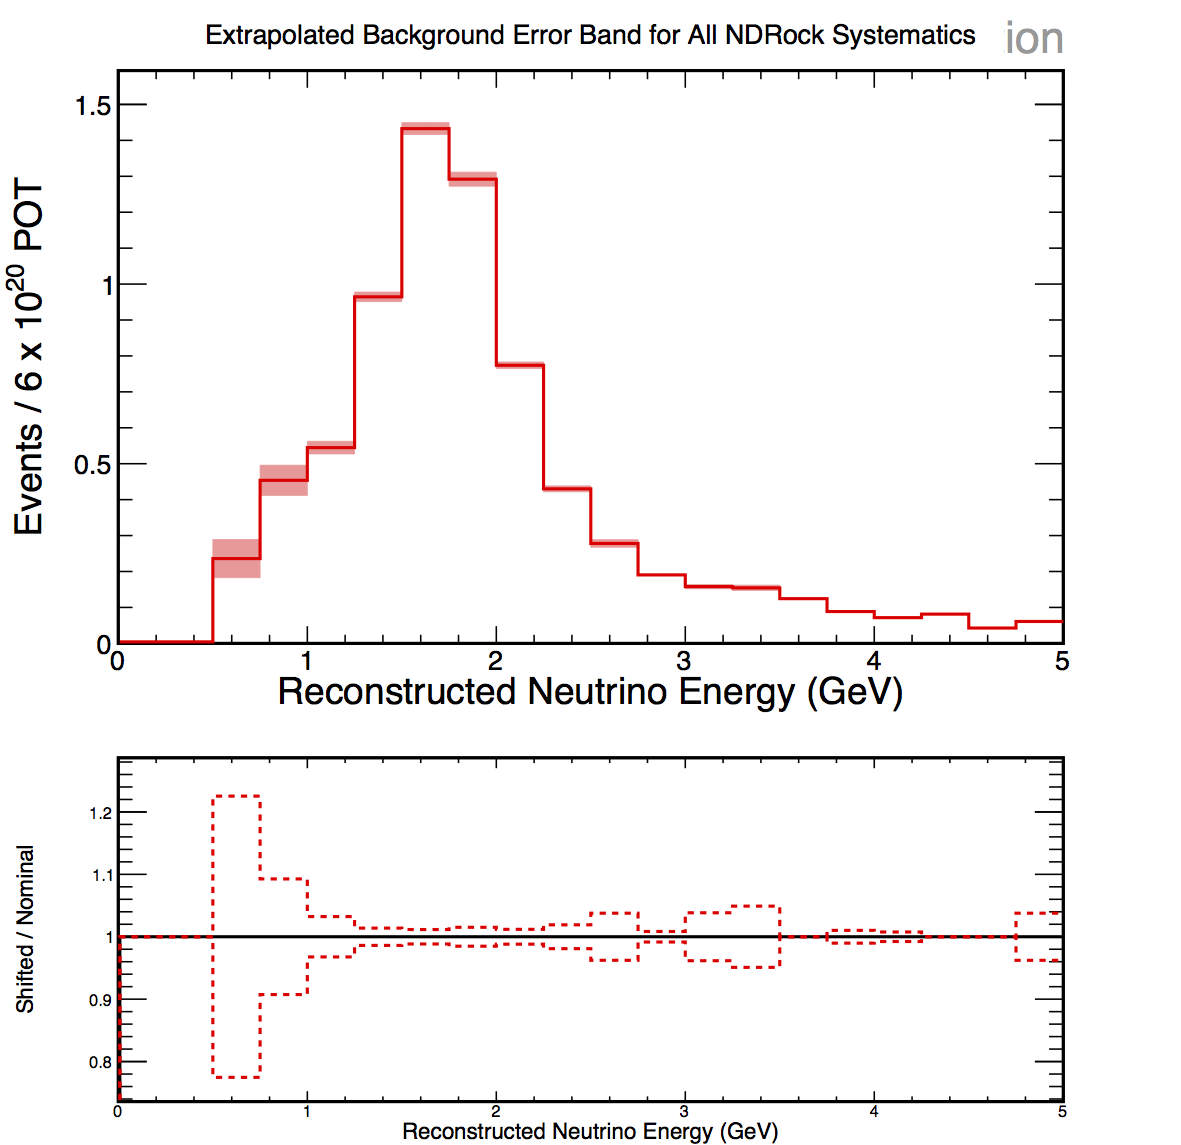
\includegraphics[width=1\linewidth]{figures/cBGEXNDRockSysts.png}
  \end{subfigure}
  \caption[ND Rock Contamination Shifted Spectra]{Shifted vs nominal spectra for the NC signal (left) and background (right). The shifted spectra are extrapolated after removal of rock events in the ND MC by truth.}
  \label{fig:SystNDRock}
\end{figure}

\section{ND Data/MC Difference and CC Background}

To assess the results over the MC simulation, data was compared to MC at the ND, and the event spectra were found to be an imperfect match; see fig.~\ref{fig:NDDataMC}. The FD prediction is made by decomposing ND data into NC, $\numu$ CC and $\nue$ CC components proportional to the amounts in the MC, so a data/MC difference can cause a systematic effect. This error was treated as a hybrid decomposition and CC background error, and as such, was quantified using a hybrid method.
\begin{figure}[h]
  \centering
  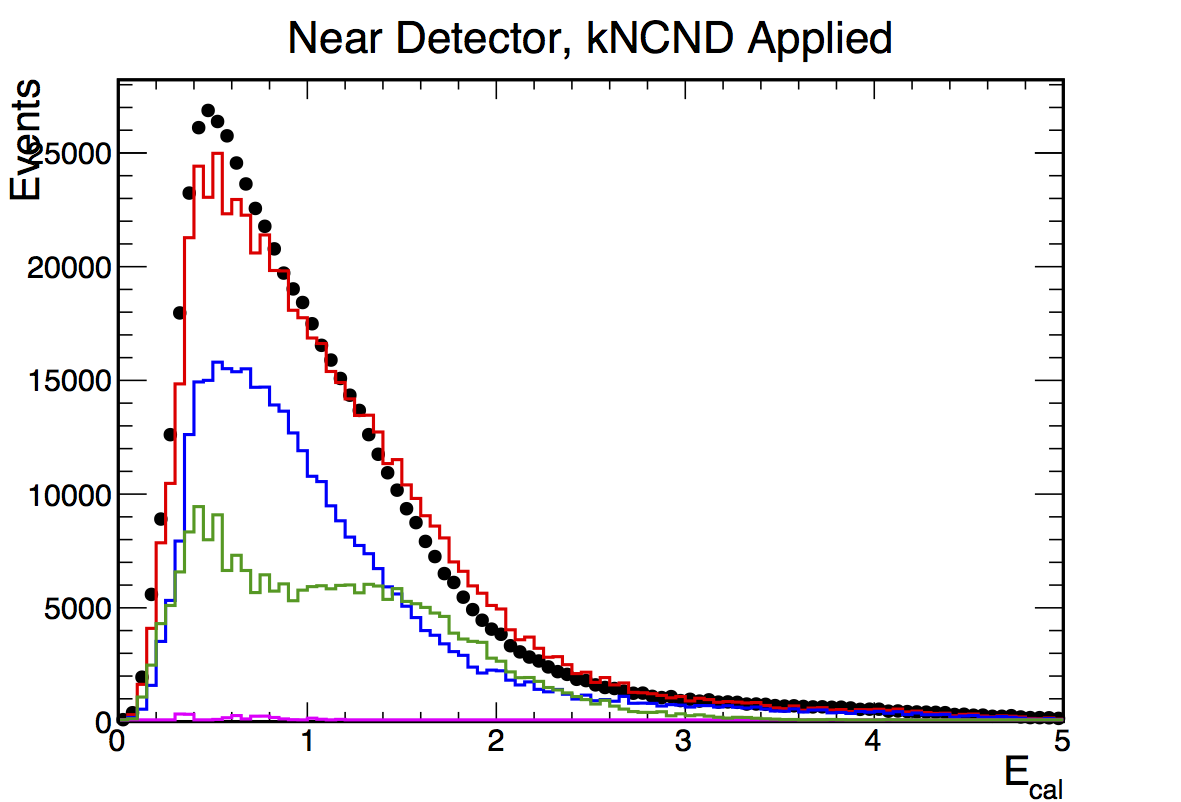
\includegraphics[width=0.75\textwidth]{figures/NDDataMC.png}
  \caption[ND Data/MC Energy Spectrum Comparison]{Energy spectra for data and MC at the ND, from ref.~\cite{ref:NDDataMC}}
  \label{fig:NDDataMC}
\end{figure}

For the first \nova~$\numu$ disappearance and $\nue$ appearance analyses, the two groups used different methods to estimate their background uncertainties. The $\numu$ analysis noted that their backgrounds were small and thus placed a $100\%$ uncertainty on each \cite{ref:NOvAFANuMu}. The $\nue$ analysis assigned any discrepancy between ND data and MC to each of the three ND background components, used each shifted decomposition to perform an extrapolation, compared the shifted predictions to nominal, and took the shift with the largest difference as the systematic error \cite{ref:NOvAFANuE}.

The NC disappearance analysis used a combination of the above techniques to evaluate the ND data/MC and CC background systematic error. The background from the beam $\nue$ component was calculated to be small, so this component was allowed to vary by $\pm100\%$. The shifted spectrum was used for extrapolation, and the percentage difference between the nominal and shifted predictions was taken as the error. For both the NC and $\numu$ CC components, the error was taken following the same procedure as the $\nue$ analysis. Results from both these two studies were then combined in quadrature. Shifting the beam $\nue$ component up and down produced the same net change in event numbers, albeit in opposite directions. Assigning the data/MC difference to the NC component caused the larger overall difference, compared to assignment to the $\numu$ CC component. The overall error was thus calculated by combining in quadrature the errors from assigning the data/MC difference to the NC component and shifting the beam $\nue$ component by $\vert 100\% \vert$, for a result of a $6.6\%$ effect on the NC signal and a $14.8\%$ effect on the CC background. Table \ref{tab:SystNDDataMC} summarizes the results from these studies, and fig.~\ref{fig:SystNDDataMC} shows the overall error envelopes.
\begin{table}[h]
  \begin{center}
    \caption[ND Data/MC and CC Background Errors]{Systematic error covering ND data/MC discrepancy and CC backgrounds. The percentage differences were calculated by shifting the ND decomposition using the listed error method, performing an extrapolation, and comparing the predicted results to nominal.}
    \label{tab:SystNDDataMC}
    \begin{tabular}{c c c}
      \hline\hline
      Error Method & NC Difference (\%) & Background Difference (\%) \\
      \hline
      Beam $\nue$ $+100\%$ & 0.00 & 10.5 \\
      Beam $\nue$ $-100\%$ & 0.00 & 10.5 \\
      ND Data/MC difference & \multirow{2}{*}{4.4} & \multirow{2}{*}{5.2} \\
      assigned to NC component \\
      ND Data/MC difference & \multirow{2}{*}{2.4} & \multirow{2}{*}{2.0} \\
      assigned to $\numu$ CC component \\
      Overall & 6.6 & 14.8 \\
      \hline
    \end{tabular}
  \end{center}
\end{table}

\begin{figure}[h]
  \centering
  \begin{subfigure}{.48\textwidth}
    \centering
    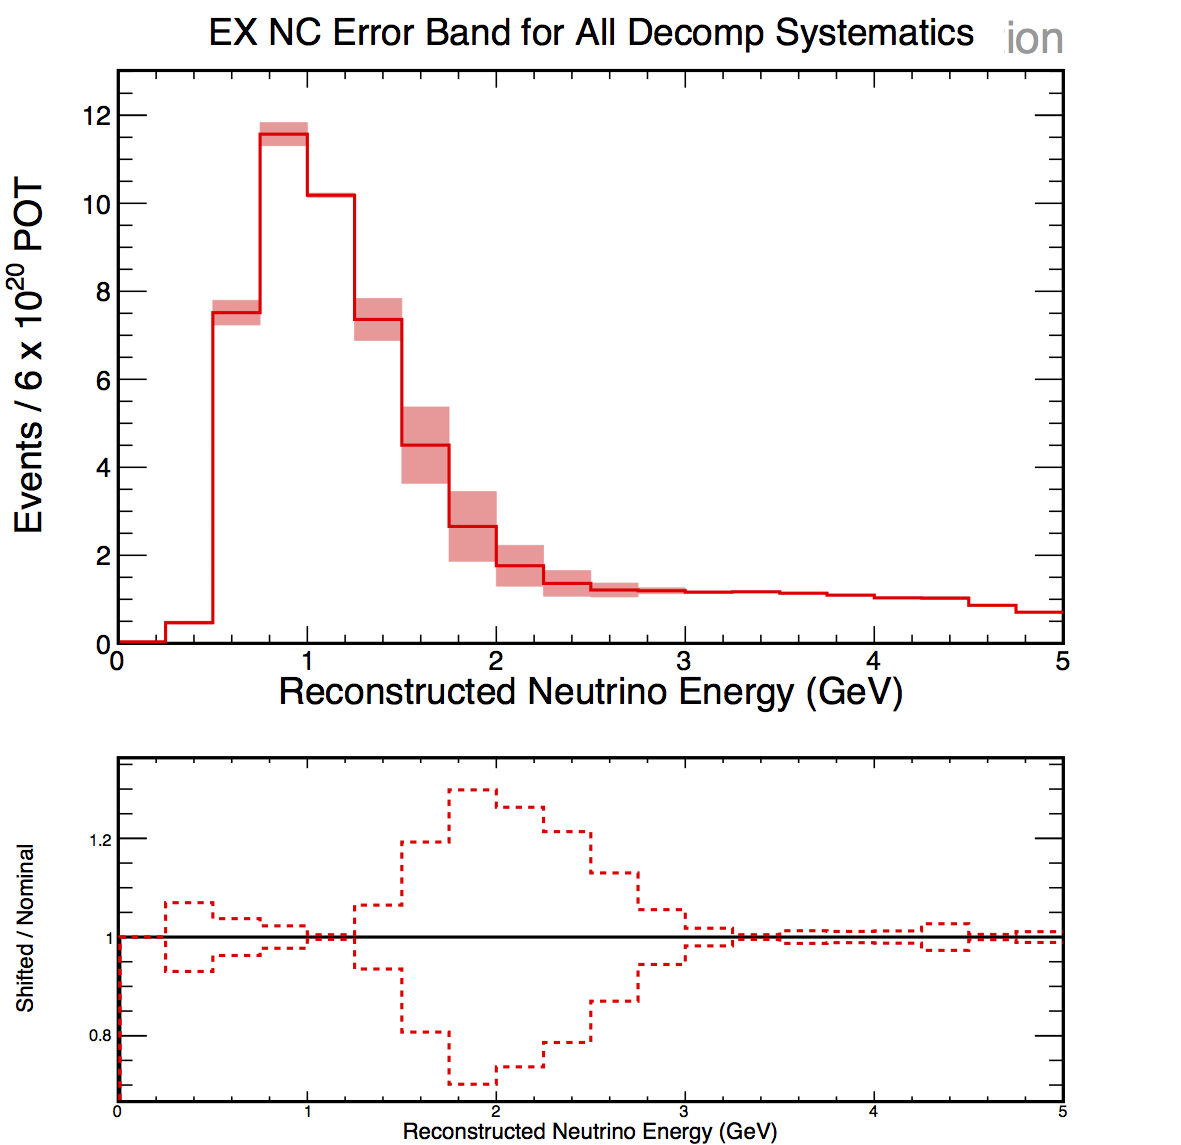
\includegraphics[width=1\linewidth]{figures/cNCEXDecompSysts.png}
  \end{subfigure}
  \begin{subfigure}{.48\textwidth}
    \centering
    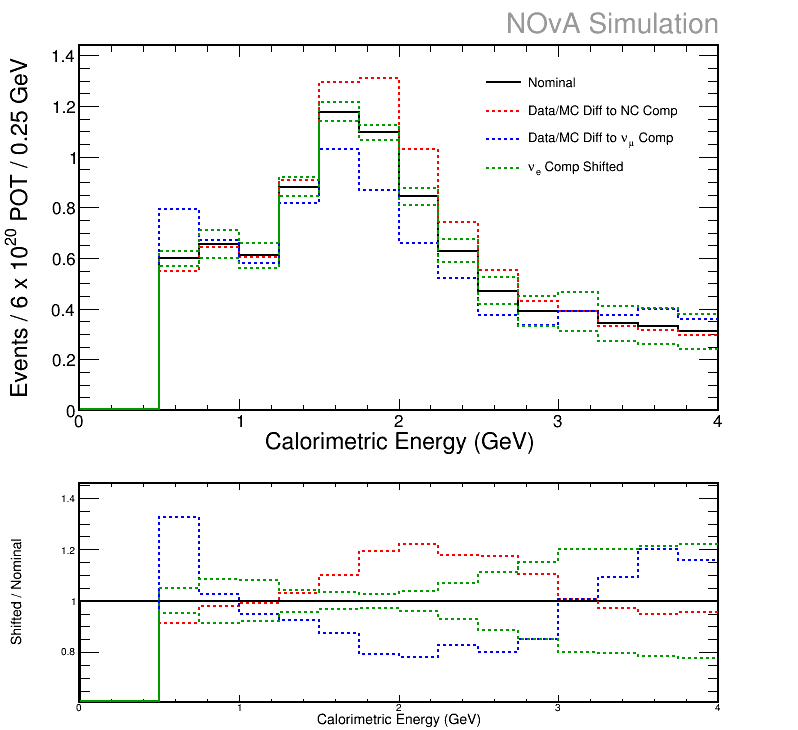
\includegraphics[width=1\linewidth]{figures/cBGEXDecompSysts.png}
  \end{subfigure}
  \caption[Systematic Error Due to ND Data/MC Discrepancy and CC Background Uncertainty]{Overall systematic error envelopes from studies to quantify ND data/MC difference and CC background uncertainties. The envelopes on the NC spectrum (left) and lower energy half of the CC background (right) are driven by the ND data/MC difference, while the high energy tail of the CC background is driven by shifting the beam $\nue$ background.}
  \label{fig:SystNDDataMC}
\end{figure}

\section{MC Statistics}

In a perfect world, there would be enough MC statistics that this section would be unnecessary, but alas, a perfect world this is not. To estimate the systematic error due to MC statistics, the MC was split into five uniformly sized samples, and each was used to extrapolate the same set of ND data. One of the resultant predicted FD spectra was labeled as nominal, and the other four were compared to this. The bin by bin differences were taken as the error between the nominal spectrum and the `shifted' spectrum. To come up with an overall uncertainty, all of the errors were added in quadrature and the result was divided by the square root of the number of samples, or $\sqrt{4} = 2$. The result was a $3.2\%$ error on the NC signal spectrum and a $5.8\%$ error on the background spectrum.

\section{Noise Model}

A sample of MC was generated for the FD using a different model of noise to study the systematic error caused by the noise model. To quantify the error, the predicted FD event spectra from the nominal and alternative MC samples were compared against each other after applying normal three flavor oscillation weights. The difference seen was $1.2\%$ for the NC signal, and $1.6\%$ for the background. As the shifted sample was only generated for the FD MC and the error was comparatively small, this systematic was added into the overall normalization.

\section{Overall Normalization}

Several independent effects contributed to an overall normalization systematic error. A $0.5\%$ error on the POT counting came from a small difference in the two toroids that determine the POT in a spill \cite{ref:TNBeam}. Uncertainties in the masses of the various parts of the \nova~detectors contributed another error of $0.7\%$ \cite{ref:MassError}. Finally, a study of the reconstruction efficiency between ND data and MC showed a $1.6\%$ difference between the number of events that get fully reconstructed \cite{ref:NDDataMCRecoEff}, which was taken directly as a contribution to the normalization error. These three effects and the noise systematic were combined in quadrature and constituted a systematic error of $2.2\%$ on the NC signal and $2.4\%$ on the background.

\section{Systematic Error Summary}

Table \ref{tab:SystSummary} shows a summary of all of the systematics, as well as an overall error. The overall error was calculated by summing the error from each row in quadrature. The final systematic error on the NC signal is $TODO\%$ and the error on the background is $TODO\%$.
\begin{table}[h]
  \begin{center}
    \caption[Systematic Error Summary]{A summary of the individual systematic errors for the NC disappearance analysis. The errors are percentage differences between the nominal and shifted predicted spectra.}
    \label{tab:SystSummary}
    \begin{tabular}{r c c}
      \hline\hline
      Systematic & NC Difference (\%) & Background Difference (\%) \\
      \hline
      Beam & 3.4 & 8.7 \\
      Birks-Chou & 2.9 & 3.1 \\
      Calibration & & \\
      GENIE & 11.3 & 12.8 \\
      ND Containment & 0.8 & 0.7 \\
      ND Rock Contamination & 4.1 & 1.5 \\
      ND Data/MC & 6.6 & 14.8 \\
      MC Statistics & 3.2 & 5.8 \\
      Overall Normalization & 2.2 & 2.4 \\
      \hline
      Combined & & \\
      \hline
    \end{tabular}
  \end{center}
\end{table}

%%\begin{table}[h]
%%  \begin{center}
%    \begin{longtable}{r l c c c}
%      \caption[GENIE Systematic Errors]{The systematic error, in percentage difference, for each GENIE systematic parameter. The description and standard deviations come from ref.~\cite{ref:GENIE}.} \tabularnewline
%      \hline\hline
%      GENIE Parameter & Description & Parameter Std. Dev. & NC Diff. (\%) & Background Diff. (\%) \endhead \\
%      \hline
%      MaNCEL & Axial mass for NC elastic & $\pm25\%$ & & \\
%      EtaNCEL & Strange axial form factor $\eta$ for NC elastic & $\pm30\%$ & & \\
%      MaCCQEshape & Normalization Factor for CCQE & & & \\
%      NormCCQE & Normalization Factor for CCQE & & & \\
%      CCQEPauliSupViaKF & CCQE Pauli suppression (via changes in Fermi level $k_F$) & $\pm35\%$ & & \\
%      VecCCQEshape & Choice of CCQE vector form factors (BBA05 $\leftrightarrow$ Dipole) & - & & \\
%      CCQEMomDistroFGtoSF & & & & \\
%      MaCCRES & Axial mass for CC resonance neutrino production & $\pm20\%$ & & \\
%      MvCCRES & Vector mass for CC resonance neutrino production & $\pm10\%$ & & \\
%      MaNCRES & Axial mass for NC resonance neutrino production & $\pm20\%$ & & \\
%      MvNCRES & Vector mass for NC resonance neutrino production & $\pm10\%$ & & \\
%      MaCOHpi & Axial mass for CC and NC coherent pion production & $\pm50\%$ & & \\
%      R0COHpi & Nuclear size param controlling $pi$ absorption in RS model & $\pm10\%$ & & \\
%      RvpCC1pi & Non-resonance bkg in $\nu p$ CC$1\pi$ reactions & $\pm50\%$ & & \\
%      RvpCC2pi & Non-resonance bkg in $\nu p$ CC$2\pi$ reactions & $\pm50\%$ & & \\
%      RvnCC1pi & Non-resonance bkg in $\nu n$ CC$1\pi$ reactions & $\pm50\%$ & & \\
%      RvnCC2pi & Non-resonance bkg in $\nu n$ CC$2\pi$ reactions & $\pm50\%$ & & \\
%      RvpNC1pi & Non-resonance bkg in $\nu p$ NC$1\pi$ reactions & $\pm50\%$ & & \\
%      RvpNC2pi & Non-resonance bkg in $\nu p$ NC$2\pi$ reactions & $\pm50\%$ & & \\
%      RvnNC1pi & Non-resonance bkg in $\nu n$ NC$1\pi$ reactions & $\pm50\%$ & & \\
%      RvnNC2pi & Non-resonance bkg in $\nu n$ NC$2\pi$ reactions & $\pm50\%$ & & \\
%      RvbarpCC1pi & Non-resonance bkg in $\bar{\nu} p$ CC$1\pi$ reactions & $\pm50\%$ & & \\
%      RvbarpCC2pi & Non-resonance bkg in $\bar{\nu} p$ CC$2\pi$ reactions & $\pm50\%$ & & \\
%      RvbarnCC1pi & Non-resonance bkg in $\bar{\nu} n$ CC$1\pi$ reactions & $\pm50\%$ & & \\
%      RvbarnCC2pi & Non-resonance bkg in $\bar{\nu} n$ CC$2\pi$ reactions & $\pm50\%$ & & \\
%      RvbarpNC1pi & Non-resonance bkg in $\bar{\nu} p$ NC$1\pi$ reactions & $\pm50\%$ & & \\
%      RvbarpNC2pi & Non-resonance bkg in $\bar{\nu} p$ NC$2\pi$ reactions & $\pm50\%$ & & \\
%      RvbarnNC1pi & Non-resonance bkg in $\bar{\nu} n$ NC$1\pi$ reactions & $\pm50\%$ & & \\
%      RvbarnNC2pi & Non-resonance bkg in $\bar{\nu} n$ NC$2\pi$ reactions & $\pm50\%$ & & \\
%      AhtBY & $A_{HT}$ higher-twist param in BY model scaling variable $\xi_w$ & $\pm25\%$ & & \\
%      BhtBY & $B_{HT}$ higher-twist param in BY model scaling variable $\xi_w$ & $\pm25\%$ & & \\
%      CV1uBY & $C_{V1u}$ u valence GRV98 PDF correction param in BY model & $\pm30\%$ & & \\
%      CV2uBY & $C_{V2u}$ u valence GRV98 PDF correction param in BY model & $\pm40\%$ & & \\
%      NormDISCC & Inclusive CC cross-section normalization factor & & & \\
%      RnubarnuCC & $\bar{\nu}/\nu$ CC ratio & & & \\
%      DISNuclMod & DIS nuclear & & & \\
%      AGKY\_xF1pi & Pion transverse momentum ($p_T$) for $N\pi$ states in AGKY & - & & \\
%      AGKY\_pT1pi & Pion Feynman x ($x_F$) for $N\pi$ states in AGKY & - & & \\
%      FormZone & Hadron formation zone & $\pm50\%$ & & \\
%      Theta\_Delta2Npi & Pion angular distribution in $\Delta \rightarrow \pi N$ (isotropic $\leftrightarrow$ RS) & - & & \\
%      BR1gamma & Branching ratio for radiative resonance decays & $\pm50\%$ & & \\
%      BR1eta & Branching ratio for single-$\eta$ resonance decays & $\pm50\%$ & & \\
%      MFP\_N & Nucelon mean free path (total rescattering probability) & $\pm20\%$ & & \\
%      FrCEx\_N & Nucleon charge exchange probability & $\pm50\%$ & & \\
%      FrElas\_N & Nucleon elastic reaction probability & $\pm30\%$ & & \\
%      FrInel\_N & Nucleon inelastic reaction probability & $\pm40\%$ & & \\
%      FrAbs\_N & Nucleon absorption probability & $\pm20\%$ & & \\
%      FrPiProd\_N & Nucleon $\pi$-production probability & $\pm20\%$ & & \\
%      MFP\_pi & $\pi$ mean free path (total rescattering probability) & $\pm20\%$ & & \\
%      FrCEx\_pi & $\pi$ charge exchange probability & $\pm50\%$ & & \\
%      FrElas\_pi & $\pi$ elastic reaction probability & $\pm10\%$ & & \\
%      FrInel\_pi & $\pi$ inelastic reaction probability & $\pm40\%$ & & \\
%      FrAbs\_pi & $\pi$ absorption probability & $\pm20\%$ & & \\
%      FrPiProd\_pi & $\pi$ $\pi$-production probability & $\pm20\%$ & & \\
%      \hline
%      \label{tab:SystGENIE}
%    \end{longtable}
%%  \end{center}
%%\end{table}